\section{Benchmark NIST-3 "Linear Elasticity"}
\label{sec:bench-3}

Linear elasticity is used extensively in structural analysis
and engineering. Linear elasticity is a simplification
of the general nonlinear equations of elasticity and is the mathematical
study of how solid objects deform and become internally
stressed due to prescribed loading conditions.
In this benchmark, we present a standard system of two
coupled equations with mixed derivative for linear elasticity
in the coupling term. This example employs the adaptive multimesh $hp$-FEM
to solve the equations.

\begin{equation} \label{crack-u}
-E \frac{1-\nu^2}{1-2\nu} \frac{\partial^{2} u}{\partial x^{2}} - E\frac{1-\nu^2}{2-2 \nu} \frac{\partial^{2} u}{\partial y^{2}}
-E \frac{1-\nu^2}{(1-2\nu)(2-2\nu)} \frac{\partial^{2} v}{\partial x \partial y} = F_{x}
\end{equation}
\begin{equation} \label{crack-v}
-E \frac{1-\nu^2}{2-2\nu} \frac{\partial^{2} v}{\partial x^{2}} - E\frac{1-\nu^2}{1-2\nu} \frac{\partial^{2} v}{\partial y^{2}}
-E \frac{1-\nu^2}{(1-2\nu)(2-2\nu)} \frac{\partial^{2} u}{\partial x \partial y} = F_{y},
\end{equation}
where $F_{x} = F_{y} = 0$, $u$ and $v$ are the
$x$ and $y$ displacements, $E$ is Young's Modulus,
and $\nu$ is Poisson's ratio.

The domain in the example is $\Omega = (-1, 1)^2$ with a slit,
equipped with Dirichlet boundary conditions given by the
exact solution. The exact solution of (\ref{crack-u})
and (\ref{crack-v}) in polar coordinates is given by

\begin{equation}\label{exact-nist-3-u-1}
u(x, y) = \frac{1}{2G} r^{\lambda}[(k - Q(\lambda + 1))cos(\lambda \theta) - \lambda cos((\lambda - 2) \theta)]
\end{equation}
\begin{equation}\label{exact-nist-3-v-1}
v(x, y) = \frac{1}{2G} r^{\lambda}[(k + Q(\lambda + 1))sin(\lambda \theta) + \lambda sin((\lambda - 2) \theta)]
\end{equation}
here $\lambda = 0.5444837367825$, $Q = 0.5430755788367$,
$k = 3 - 4 \nu$ and $G = E / (2(1 + \nu))$.
The solution of NIST-3 is shown in Fig. \ref{fig:sln-nist03}.

\begin{figure}[!ht]
\centering
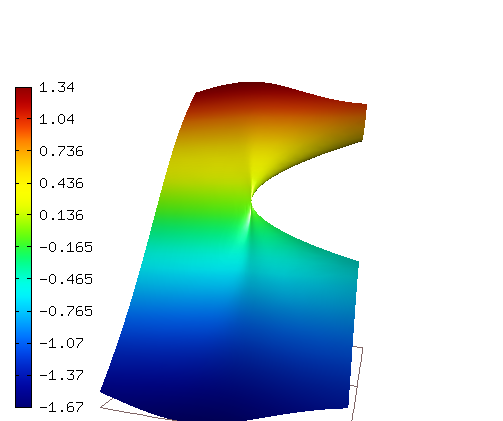
\includegraphics[height=40mm]{nist/nist-3/solution-u.png}\ \
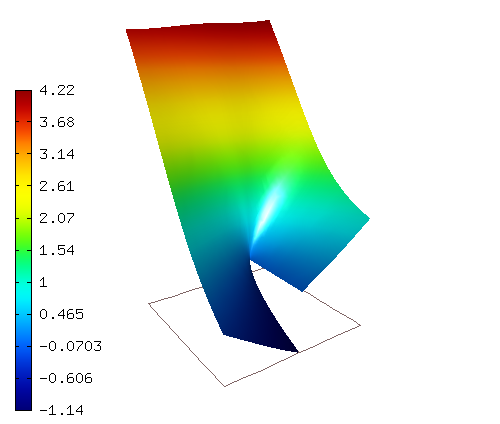
\includegraphics[height=40mm]{nist/nist-3/solution-v.png}
\vspace{-2mm}
\caption{The $u$ (left) and $v$ (right) component to NIST-3 benchmark problem.}
\label{fig:sln-nist03}
\end{figure}

The goal of the benchmark is to reach a relative error below
$10^{-1}$~\% in the $H^1$-norm with as few DOFs as possible.
We begin with adaptive $hp$-FEM with possible anisotropic refinements.
The initial mesh is shown in Fig. \ref{fig:nist-3-hp-aniso-init}.
In a few adaptivity steps, the polynomial degree of elements is increased
anisotropically.

\begin{figure}[!ht]
\centering
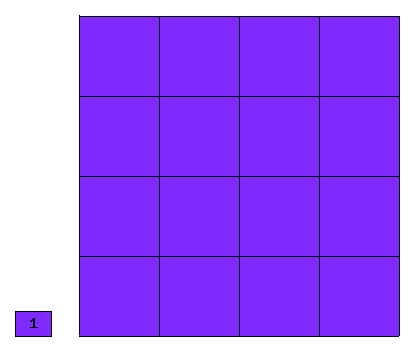
\includegraphics[height=5cm]{nist/nist-3/mesh_hp_aniso_init.png}
\caption{Initial mesh.}
\label{fig:nist-3-hp-aniso-init}
\end{figure}

The resulting mesh with 3897 DOF is shown in Fig. \ref{fig:nist-3-hp-aniso}.

\begin{figure}[!ht]
\centering
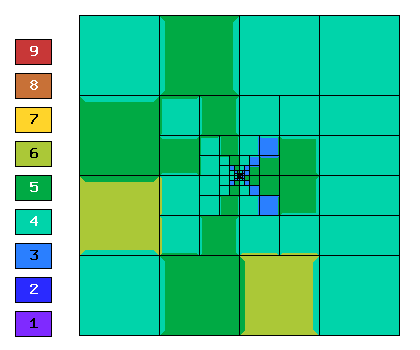
\includegraphics[height=5cm]{nist/nist-3/mesh_u_hp_anisoh.png}\ \
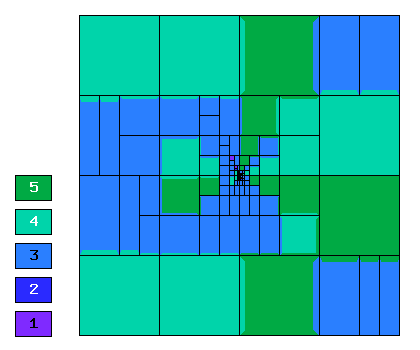
\includegraphics[height=5cm]{nist/nist-3/mesh_v_hp_anisoh.png}
\vspace{-2mm}
\caption{Final meshs of $u$ (left) and $v$ (right) component for $hp$-FEM with anisotropic refinements.}
\label{fig:nist-3-hp-aniso}
\end{figure}

The final relative error estimate in $H^1$-norm was 8.05635e-02 \%,
and it was identical to the exact error in all printed digits.
We also solved this benchmark with adaptive $h$-FEM
with linear and quadratic elements, with anisotropic refinements enabled.
Final meshes for the $h$-FEM computations are shown
in Fig. \ref{fig:nist-3-h1-aniso} and Fig. \ref{fig:nist-3-h2-aniso}.

\begin{figure}[!ht]
\centering
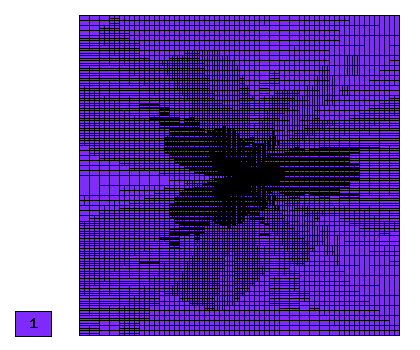
\includegraphics[height=5cm]{nist/nist-3/mesh_u_h1_aniso.png}\ \
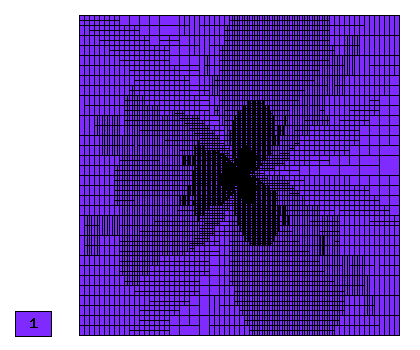
\includegraphics[height=5cm]{nist/nist-3/mesh_v_h1_aniso.png}
\caption{Final meshs of $u$ (left) and $v$ (right) component for $h$-FEM anisotropic refinements with linear elements.}
\label{fig:nist-3-h1-aniso}
\end{figure}

\begin{figure}[!ht]
\centering
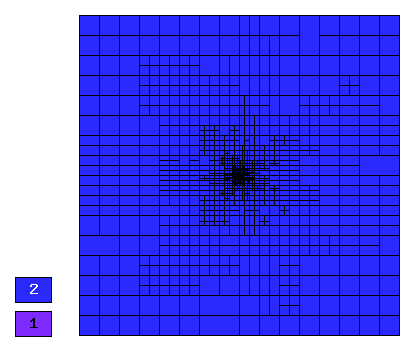
\includegraphics[height=5cm]{nist/nist-3/mesh_u_h2_aniso.png}\ \
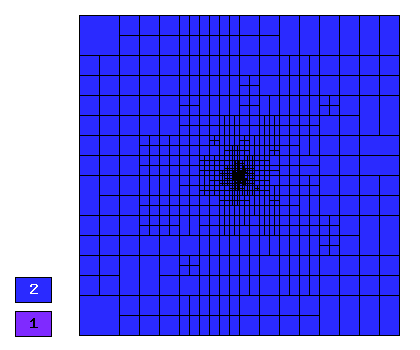
\includegraphics[height=5cm]{nist/nist-3/mesh_v_h2_aniso.png}
\caption{Final meshs of $u$ (left) and $v$ (right) component for $h$-FEM anisotropic refinements with quadratic elements.}
\label{fig:nist-3-h2-aniso}
\end{figure}

Figs. \ref{fig:nist-3-conv} compare all
three approaches to automatic adaptivity from the point
of view of DOF and CPU convergence.

\begin{figure}[!ht]
\centering
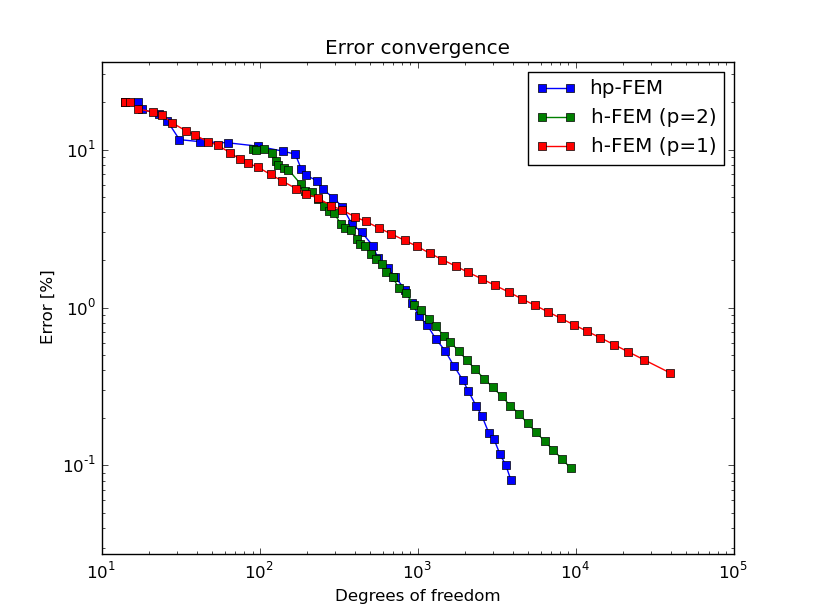
\includegraphics[height=5cm]{nist/nist-3/conv_dof_aniso.png}\ \
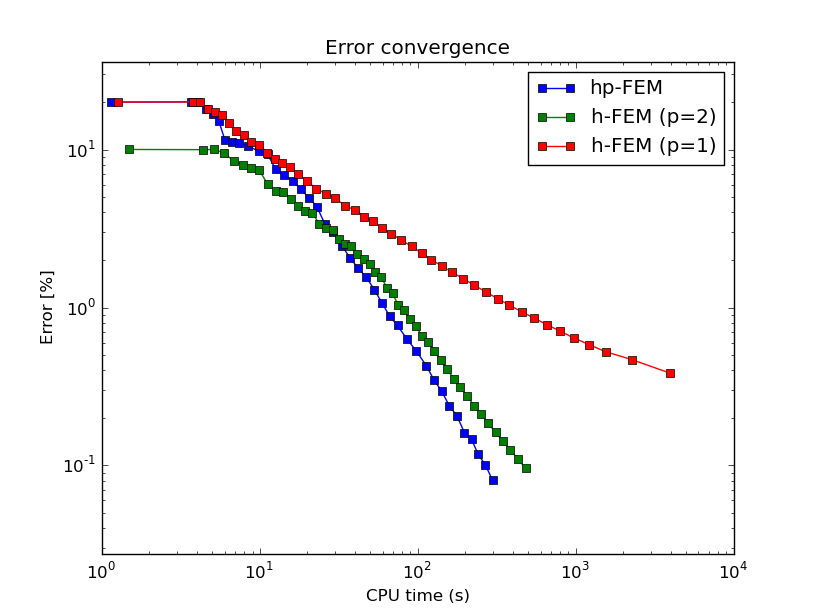
\includegraphics[height=5cm]{nist/nist-3/conv_cpu_aniso.png}
\caption{DOF and CPU time convergence graphs.}
\label{fig:nist-3-conv}
\end{figure}

